\let\negmedspace\undefined
\let\negthickspace\undefined
\documentclass[journal]{IEEEtran}
\usepackage[a5paper, margin=10mm, onecolumn]{geometry}
%\usepackage{lmodern} % Ensure lmodern is loaded for pdflatex
\usepackage{tfrupee} % Include tfrupee package

\setlength{\headheight}{1cm} % Set the height of the header box
\setlength{\headsep}{0mm}     % Set the distance between the header box and the top of the text

\usepackage{gvv-book}
\usepackage{gvv}
\usepackage{cite}
\usepackage{amsmath,amssymb,amsfonts,amsthm}
\usepackage{algorithmic}
\usepackage{graphicx}
\usepackage{textcomp}
\usepackage{xcolor}
\usepackage{txfonts}
\usepackage{listings}
\usepackage{enumitem}
\usepackage{mathtools}
\usepackage{gensymb}
\usepackage{comment}
\usepackage[breaklinks=true]{hyperref}
\usepackage{tkz-euclide} 
\usepackage{listings}
% \usepackage{gvv}                                        
\def\inputGnumericTable{}                                 
\usepackage[latin1]{inputenc}                                
\usepackage{color}                                            
\usepackage{array}                                            
\usepackage{longtable}                                       
\usepackage{calc}                                             
\usepackage{multirow}                                         
\usepackage{hhline}                                           
\usepackage{ifthen}                                           
\usepackage{lscape}
\begin{document}

\bibliographystyle{IEEEtran}
\vspace{3cm}

\title{2.10.41}
\author{EE25BTECH11012-BEERAM MADHURI}
% \maketitle
% \newpage
% \bigskip
{\let\newpage\relax\maketitle}

\renewcommand{\thefigure}{\theenumi}
\renewcommand{\thetable}{\theenumi}
\setlength{\intextsep}{10pt} % Space between text and floats


\numberwithin{equation}{enumi}
\numberwithin{figure}{enumi}
\renewcommand{\thetable}{\theenumi}


\textbf{Question}:\\
Let the vectors $\mathbf{a}, \mathbf{b}, \mathbf{c}$ and $\mathbf{d}$ be such that $(\mathbf{a} \times \mathbf{b}) \times (\mathbf{c} \times \mathbf{d}) = \mathbf{0}$. Let $A$ and $B$ be planes determined by the pairs of vectors $\mathbf{a}, \mathbf{b}$ and $\mathbf{c}, \mathbf{d}$ respectively. Then the angle between $A$ and $B$ is

\begin{enumerate}
\begin{multicols}{4}
\item[a)] $0$
\item[b)] $\frac{\pi}{4}$
\item[c)] $\frac{\pi}{3}$
\item[d)] $\frac{\pi}{2}$
\end{multicols}
\end{enumerate}
\textbf{Solution}:\\
given, 
\begin{align}
(\mathbf{a} \times \mathbf{b}) \times (\mathbf{c} \times \mathbf{d}) = 0
\end{align}
\begin{align*}
A &: \text{span of } \vec{a}, \vec{b} \\
B &: \text{span of } \vec{c}, \vec{d}
\end{align*}

Cross product of 2 vectors can be written using a skew-symmetric matrix:
\begin{align}
\vec{a} \times \vec{b} = [\vec{a}]_{\times} \vec{b} \quad \text{where} \quad [\vec{a}]_{\times} = \begin{bmatrix}0 & -a_3 & a_2 \\a_3 & 0 & -a_1 \\-a_2 & a_1 & 0\end{bmatrix}
\end{align}
Thus,
\begin{align}
(\vec{a} \times \vec{b}) \times (\vec{c} \times \vec{d}) = [\vec{a} \times \vec{b}]_{\times}(\vec{c} \times \vec{d}) = 0\\
[\vec{a} \times \vec{b}]_{\times}(\vec{c} \times \vec{d}) = 0 \iff (\vec{c} \times \vec{d}) \parallel (\vec{a} \times \vec{b})\\
(\vec{a} \times \vec{b}) = \lambda(\vec{c} \times\vec{d})
\end{align}
normals to planes A and B:
\begin{align}
n_A = \mathbf{a} \times \mathbf{b}\\
n_B = \mathbf{c} \times \mathbf{d}\\
n_A = \lambda n_B
\end{align}

Angle between Planes A and B = Angle between Normals $n_A$ and $n_B$\\
Angle between planes A and B:
\begin{align}
\theta = \cos^{-1}\!\left(
\frac{\mathbf{n}_A^\top \mathbf{n}_B}{\|\mathbf{n}_A\|\,\|\mathbf{n}_B\|}
\right)\\
= \cos^{-1}\!\left(
\frac{\lambda\|\mathbf{n}_B\|^2}{|\lambda|\|\mathbf{n}_B\|^2}
\right)\\
= \cos^{-1}(\pm 1)\\
\end{align}
Considering acute angle,
\begin{align}
\theta=0\\
\therefore n_A \parallel n_B\\
\therefore plane A \parallel plane B
\end{align}
Hence, Angle between the planes is $0$.\\option (a).
\begin{figure}[H]
    \centering
    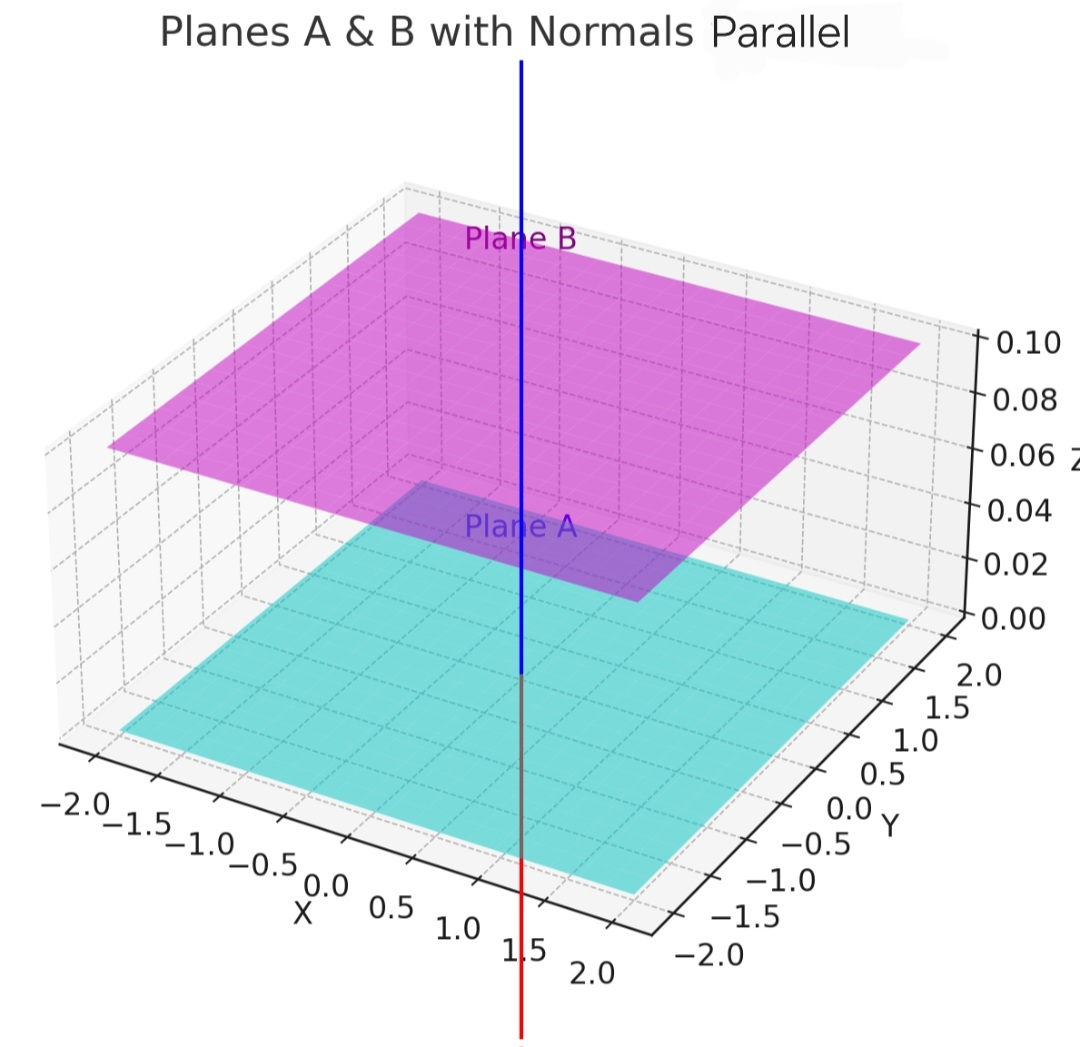
\includegraphics[width=0.75\columnwidth]{figs/graph .jpg}
    \caption{Planes A and B}
    \label{fig:placeholder}
\end{figure}

\end{document}